\documentclass[11pt, oneside]{article} 
\usepackage{geometry}
\geometry{letterpaper} 
\usepackage{graphicx}
	
\usepackage{amssymb}
\usepackage{amsmath}
\usepackage{parskip}
\usepackage{color}
\usepackage{hyperref}

\graphicspath{{/Users/telliott_admin/Tex/png/}}
% \begin{center} 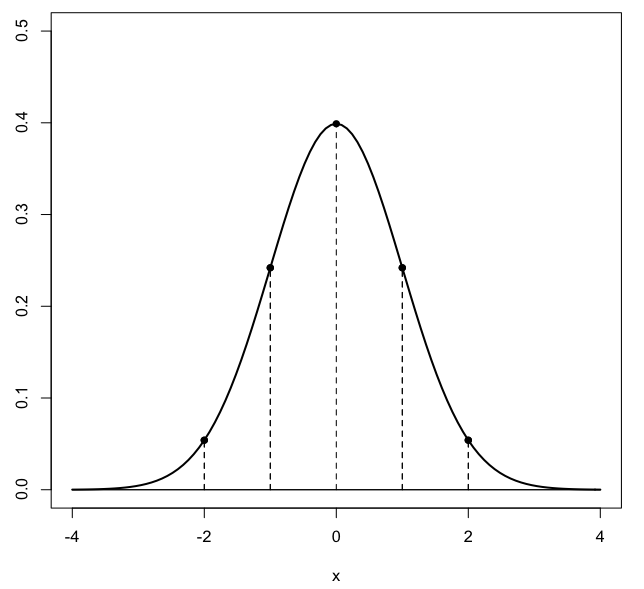
\includegraphics [scale=0.4] {gauss3.png} \end{center}

\title{Headlight problem}
\date{}

\begin{document}
\maketitle
\Large

The reflective property of the parabola asserts that if a light ray emitted from the focus bounces off any point of the parabola, it then travels off in the vertical direction.

Snell's law for reflection says that the angle of incidence and reflection to the inside surface of the parabola must be equal.  It is curious that this law has Snell's name on it, since the fact was known to Euclid, and Heron had a proof of it.  The proof depends on the assumption that light travels the shortest path between two points.

In any case, applying that law to this problem, the angle of incidence is the angle of the magenta vector $\mathbf{w}$ with the tangent vector $\mathbf{u}$.  This is equal to the angle of reflection, the angle of the tangent $\mathbf{u}$ with the vertical vector $\mathbf{v}$.

\begin{center} 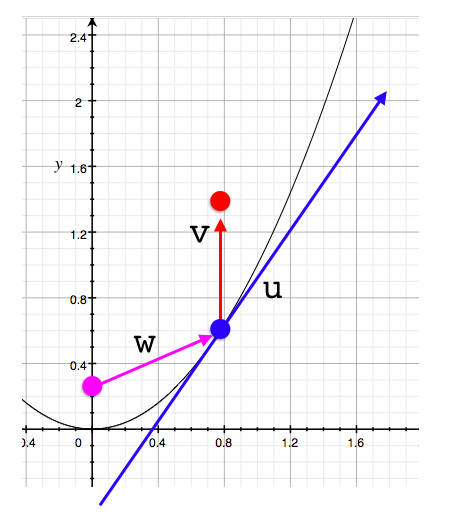
\includegraphics [scale=0.4] {headlight.png} \end{center}

We assert that there exists a point on the $y$-axis (the focus, colored magenta), with the property that when we draw a vector to any point on the parabola, the angle that this vector makes with the tangent to the parabola is equal to the angle the tangent makes with the vertical.

Let the distance of this point from the origin be $p$.  Then
\[ \mathbf{w} = \langle x, ax^2 - p \rangle \]

The tangent has slope $2ax$ so 
\[ \mathbf{u} = \langle 1, 2ax \rangle \]

Scale the vertical to be a unit vector
\[ \mathbf{v} = \langle 0, 1 \rangle \]

By the definition of the dot product, the cosine of the angle between $\mathbf{w}$ and $\mathbf{u}$ is
\[ \frac{\mathbf{w} \cdot \mathbf{u}}{u \ w} \]

By the equal angle constraint, this is equal to the cosine of the angle between $\mathbf{u}$ and $\mathbf{v}$
\[ \frac{\mathbf{u} \cdot \mathbf{v}}{u \ v} = \frac{\mathbf{w} \cdot \mathbf{u}}{u \ w} \]
Since $v = 1$ we have
\[ w \ ( \mathbf{u} \cdot \mathbf{v} ) = \mathbf{w} \cdot \mathbf{u} \]

That's the important logic of the solution.

Now it's just algebra:
The length of $\mathbf{w}$ is 
\[ w = \sqrt{x^2 + (ax^2 - p)^2} \]
while
\[  \mathbf{u} \cdot \mathbf{v} = 2ax \]
\[  \mathbf{w} \cdot \mathbf{u} =  x + 2ax(ax^2 - p) \]

So
\[ w \ ( \mathbf{u} \cdot \mathbf{v} ) = \mathbf{w} \cdot \mathbf{u} \]
\[ \sqrt{x^2 + (ax^2 - p)^2} \ (2ax) = x + 2ax(ax^2 - p) \]
Divide by $2ax$:
\[ \sqrt{x^2 + (ax^2 - p)^2} = \frac{1}{2a} + (ax^2 - p) \]
Square both sides
\[ x^2 + (ax^2 - p)^2 = \frac{1}{(2a)^2} + \frac{1}{a}(ax^2 - p) +  (ax^2 - p)^2 \]
A nice cancelation:
\[ x^2 = \frac{1}{(2a)^2} + \frac{1}{a}(ax^2 - p)  \]
We can also cancel the $x^2$:
\[ 0 = \frac{1}{(2a)^2} + \frac{1}{a}( - p)  \]
and finally cancel an $a$:
\[ 0 = \frac{1}{4a}  - p \]
\[ p = \frac{1}{4a} \]

The point $(0, 1/4a)$ is, as we saw before, the focus of the parabola.

Since $p$ is independent of $x$, this property holds for every point on the parabola.  

\begin{center} 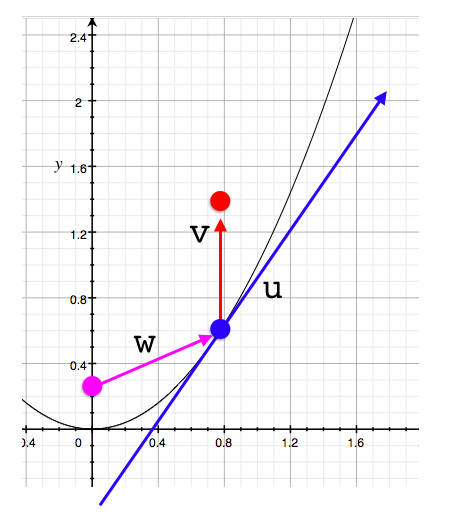
\includegraphics [scale=0.4] {headlight.png} \end{center}
An alternative, more geometric approach is to note that the angle the vector $\mathbf{u}$ makes with the vertical at $(x, ax^2)$ is equal to the angle $\mathbf{u}$ makes with the $y$-axis (just off the image to the bottom).

This angle is equal to the angle between $\mathbf{w}$ and $\mathbf{u}$ if and only if the triangle is isosceles, that is, if length of the vector $\mathbf{w}$ is equal to the distance between $(0,p)$ and the intersection of $\mathbf{u}$ with the $y$-axis.  

We start by exploring the properties of a line through the point $(x, ax^2)$ with slope equal to $2ax$.  

From this point on, the point on the parabola is \emph{fixed}.  We want to write an equation for a line with the same slope as the parabola at this point, the same slope as the vector $\mathbf{u}$.

We will be re-using $x$ as a variable.  To reduce confusion, label the fixed value at the point as $\hat{x}$, so then $\hat{y} = a\hat{x}^2$, and the slope is $2a \hat{x}$.

The point-slope formula for the line is 
\[ 2a \hat{x} = \frac{\Delta y}{\Delta x} = \frac{y - \hat{y}}{x - \hat{x}} =  \frac{y - a \hat{x}^2}{x - \hat{x}} \]

The intersection with the $y$-axis occurs at $y = 0$ so there
\[ 2a \hat{x} = \frac{- a \hat{x}^2}{x - \hat{x}} \]
\[ 2 = \frac{- \hat{x}}{x - \hat{x}} \]
\[ 2x - 2 \hat{x} = - \hat{x} \]
\[ x = \frac{\hat{x}}{2} \]
The intersection of $\mathbf{u}$ with the $x$-axis is at $\hat{x}/2$.

For the intersection with the $y$-axis, $x = 0$ and then
\[ 2a \hat{x} = \frac{y - a \hat{x}^2}{- \hat{x}} \]
\[ -2a \hat{x}^2 = y - a \hat{x}^2 \]
\[ y = - a \hat{x}^2 \]

What we've discovered is that the point of intersection is the same distance below the $x$-axis as our point on the parabola $(\hat{x}, a\hat{x}^2)$ is above it.  We could have used congruent triangles proceeding from the discovery above that the intersection of with the $x$-axis is at $\hat{x}/2$.

Our goal is to show that the triangle is isosceles:
\[ a\hat{x}^2 + p = w \]
\[ a\hat{x}^2 + p = \sqrt{\hat{x}^2 + (a\hat{x}^2 - p)^2} \]
\[ (a\hat{x}^2 + p)^2 = \hat{x}^2 + (a\hat{x}^2 - p)^2 \]
Continuing
\[ a^2 \hat{x}^4 + 2ap \hat{x}^2 + p^2 = \hat{x}^2 + a^2 \hat{x}^4 - 2ap \hat{x}^2 + p^2 \]
Does this look familiar?

Cancel two terms
\[ 2ap \hat{x}^2 = \hat{x}^2  - 2ap \hat{x}^2 \]
\[ 4ap\hat{x}^2 = \hat{x}^2 \]
\[ 4ap = 1 \]
\[ p = \frac{1}{4a} \]
And we already proved this is true, if the magenta point we start from is the focus.

Hence the lengths are equal, the triangle is isosceles, and the corresponding angles are equal.  The point we've been using is just the focus.

\end{document} 